\documentclass[10pt,a4paper]{article}
\usepackage[utf8]{inputenc}
\usepackage{amsmath}
\usepackage{amsfonts}
\usepackage{amssymb}
\usepackage{graphicx}
\usepackage{enumerate}
\begin{document}

\section{Set Theory}

x

To demystify mathematics consider
\begin{enumerate}[(i)]
\item What is a theorem?
\item What is a proof?
\end{enumerate}
What if we don't know the answer?

To begin we need
\begin{enumerate}[(a)]
\item an example(s)
\item a nearly related concept
\end{enumerate}


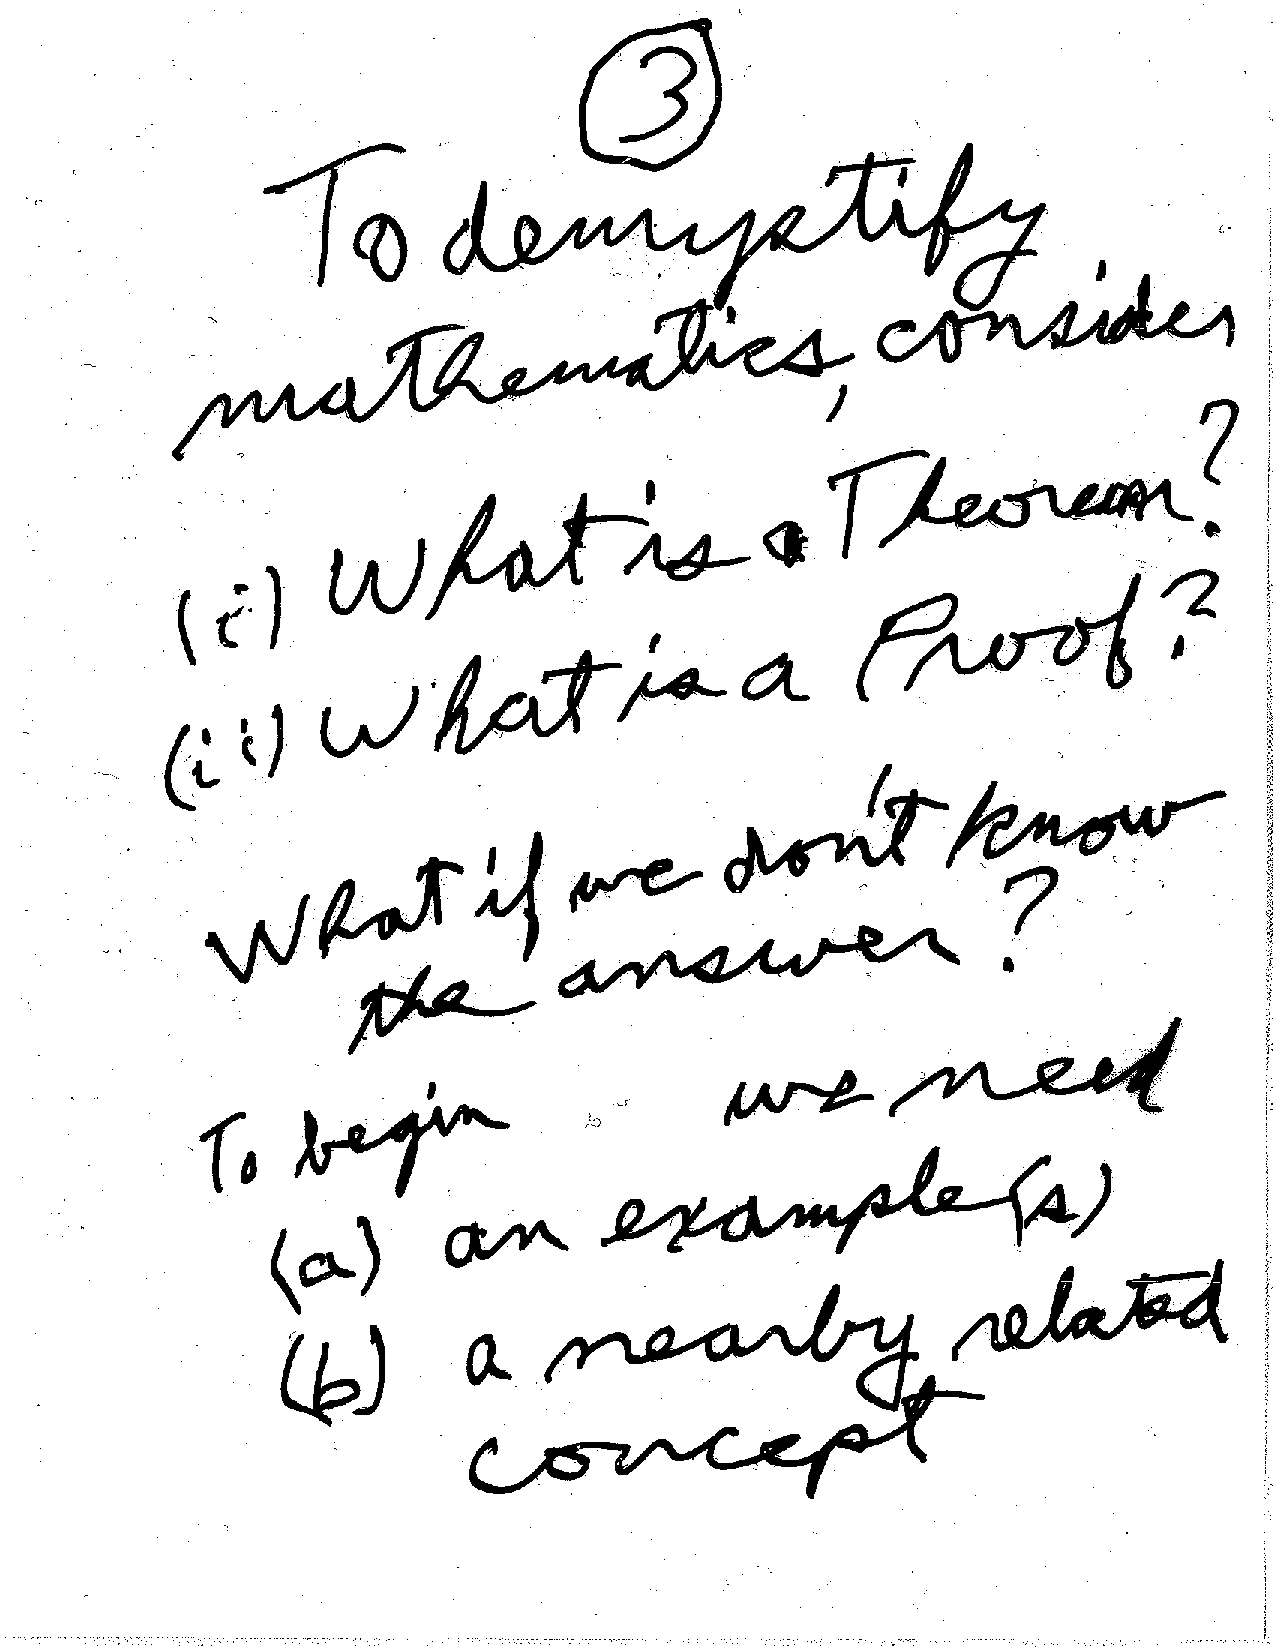
\includegraphics[scale=.5]{Pages/ST_3}

\newpage

Related Concept: Greek Syllogism

\underline{example:}
\begin{enumerate}
\item All men are mortal.
\item Socrates is a man.
\item Therefore, Socrates must die. 
\end{enumerate}

To analyze, recast in set theoretic terms via Venn Diagram.

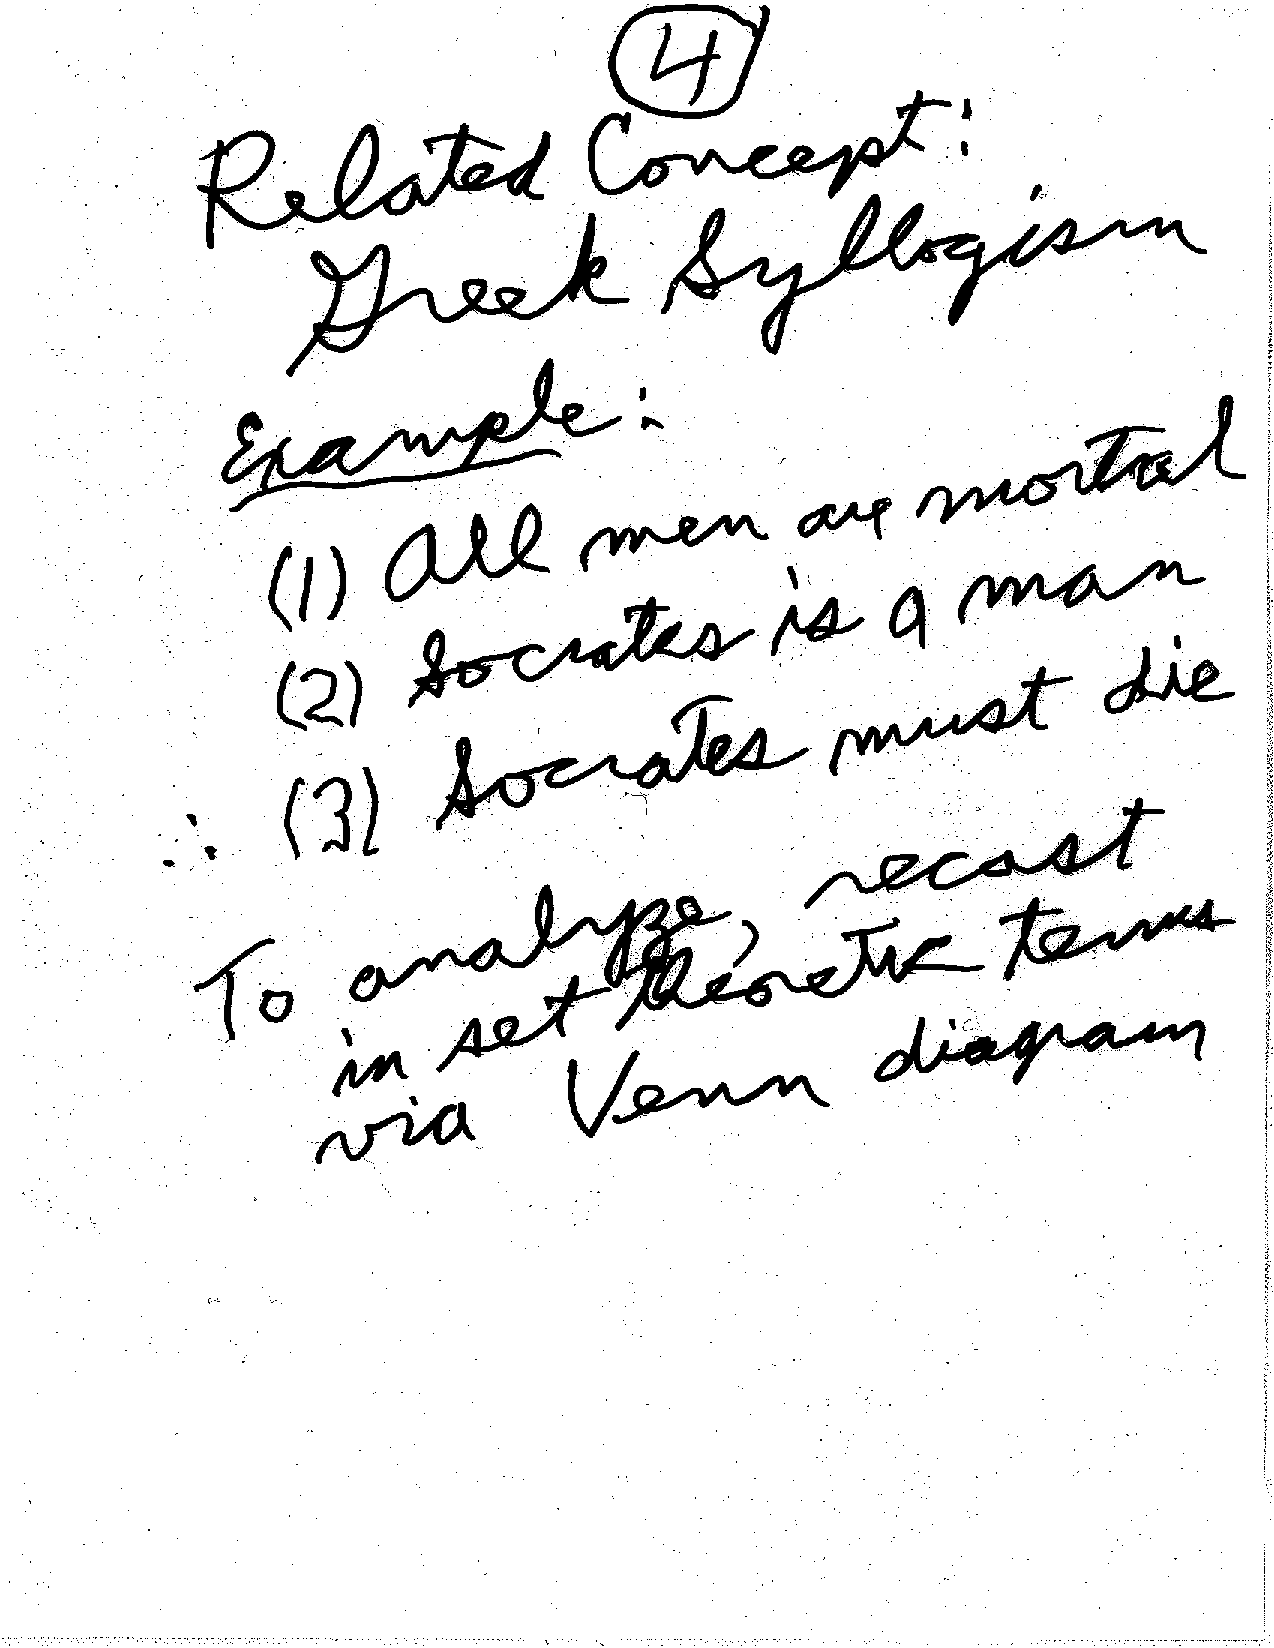
\includegraphics[scale=.5]{Pages/ST_4}

\newpage

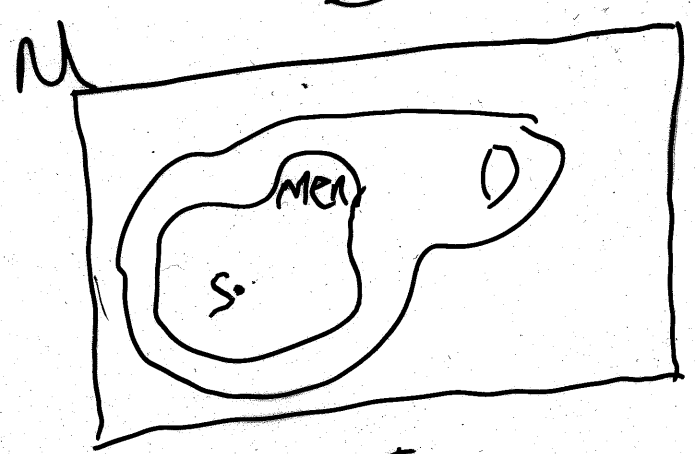
\includegraphics[scale=.2]{Pages/ST_5_im1}

$S$: Socrates\\
$M$: Set of Men\\
$D$: Things that will die\\
$\mathcal{U}$: Things on Earth

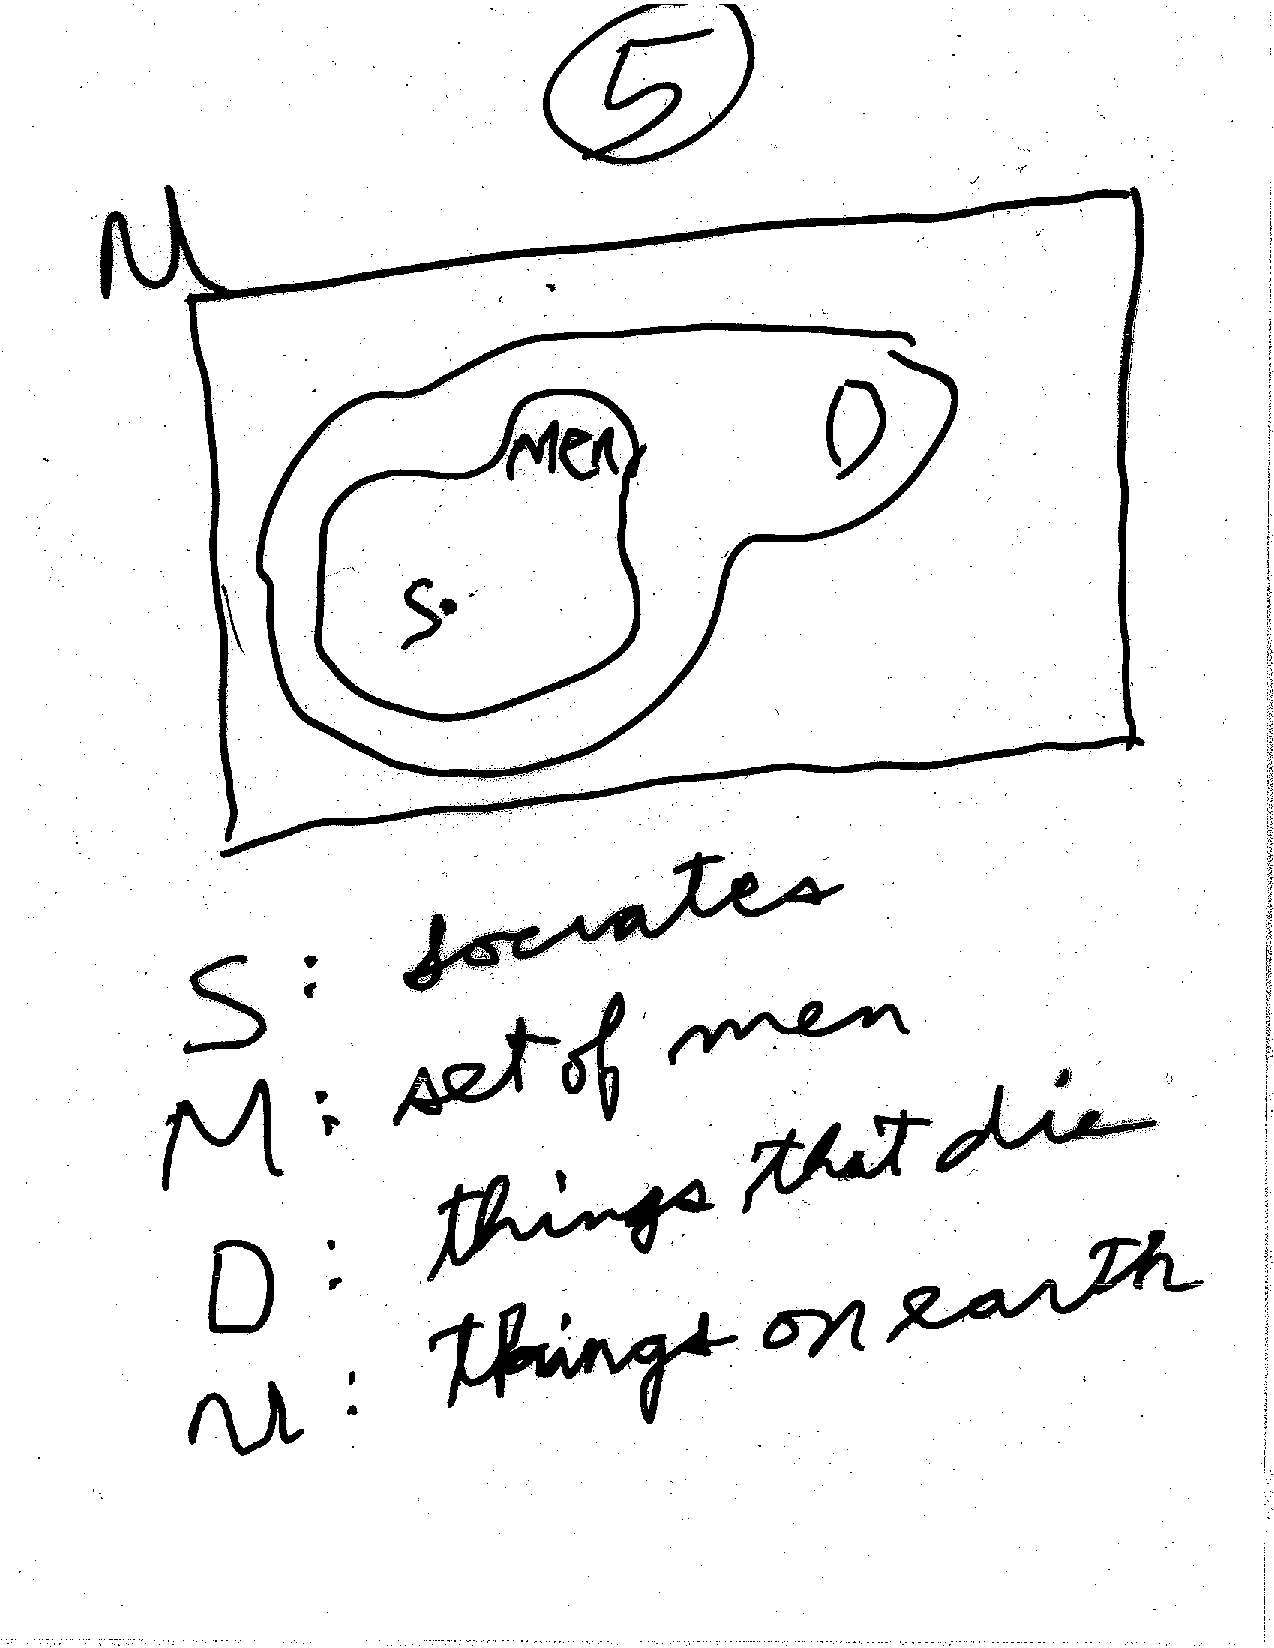
\includegraphics[scale=.5]{Pages/ST_5} 



%Zack: Pages 6,7,8,19,20

%Jack: 21, 9, 10, 11

%Koka: Pages 13, 13A, 22 ,22A, 22B


\section{Generate $\mathbb{N}$}


%Ruth: Pages L4A-L4G




\section{From $\mathbb{Z}$ to $\mathbb{R}$ via ordering}
%Jazz: ZR1-ZR5

%Kyler: ZR6 - ZR10

%Preethika: ZR11-ZR14


\section{Sequence and Limits}

%Aaron: First 2 pages and 48-50

%Hamza: 51-52B

\section{Limit and Convergence}

%Joe: 50-51

%Quinten: 52-53

%Farishta: 53A-54A

\section{Infinite Series}

%Sukhreet: IS1 - IS 7

%Matthew: IS8 - IS15
\newpage
\begin{center}
IS8
\end{center}

The most definitive statement that can be made concerning whether a series can converge or diverge is based on the following so-called \underline{Cauchy Criterion}.

\underline{Theorem}
$\sum_{j=1}^{\infty}a_j$ converges if and only if  $\forall \in >$ 0 $\exists$ N $< \infty$ 

Such that for all n $\ge$ N and 0 $\le$ k $< \infty$

$|a_n + a_{n+1} + ... + a_{n+k}| < \in$

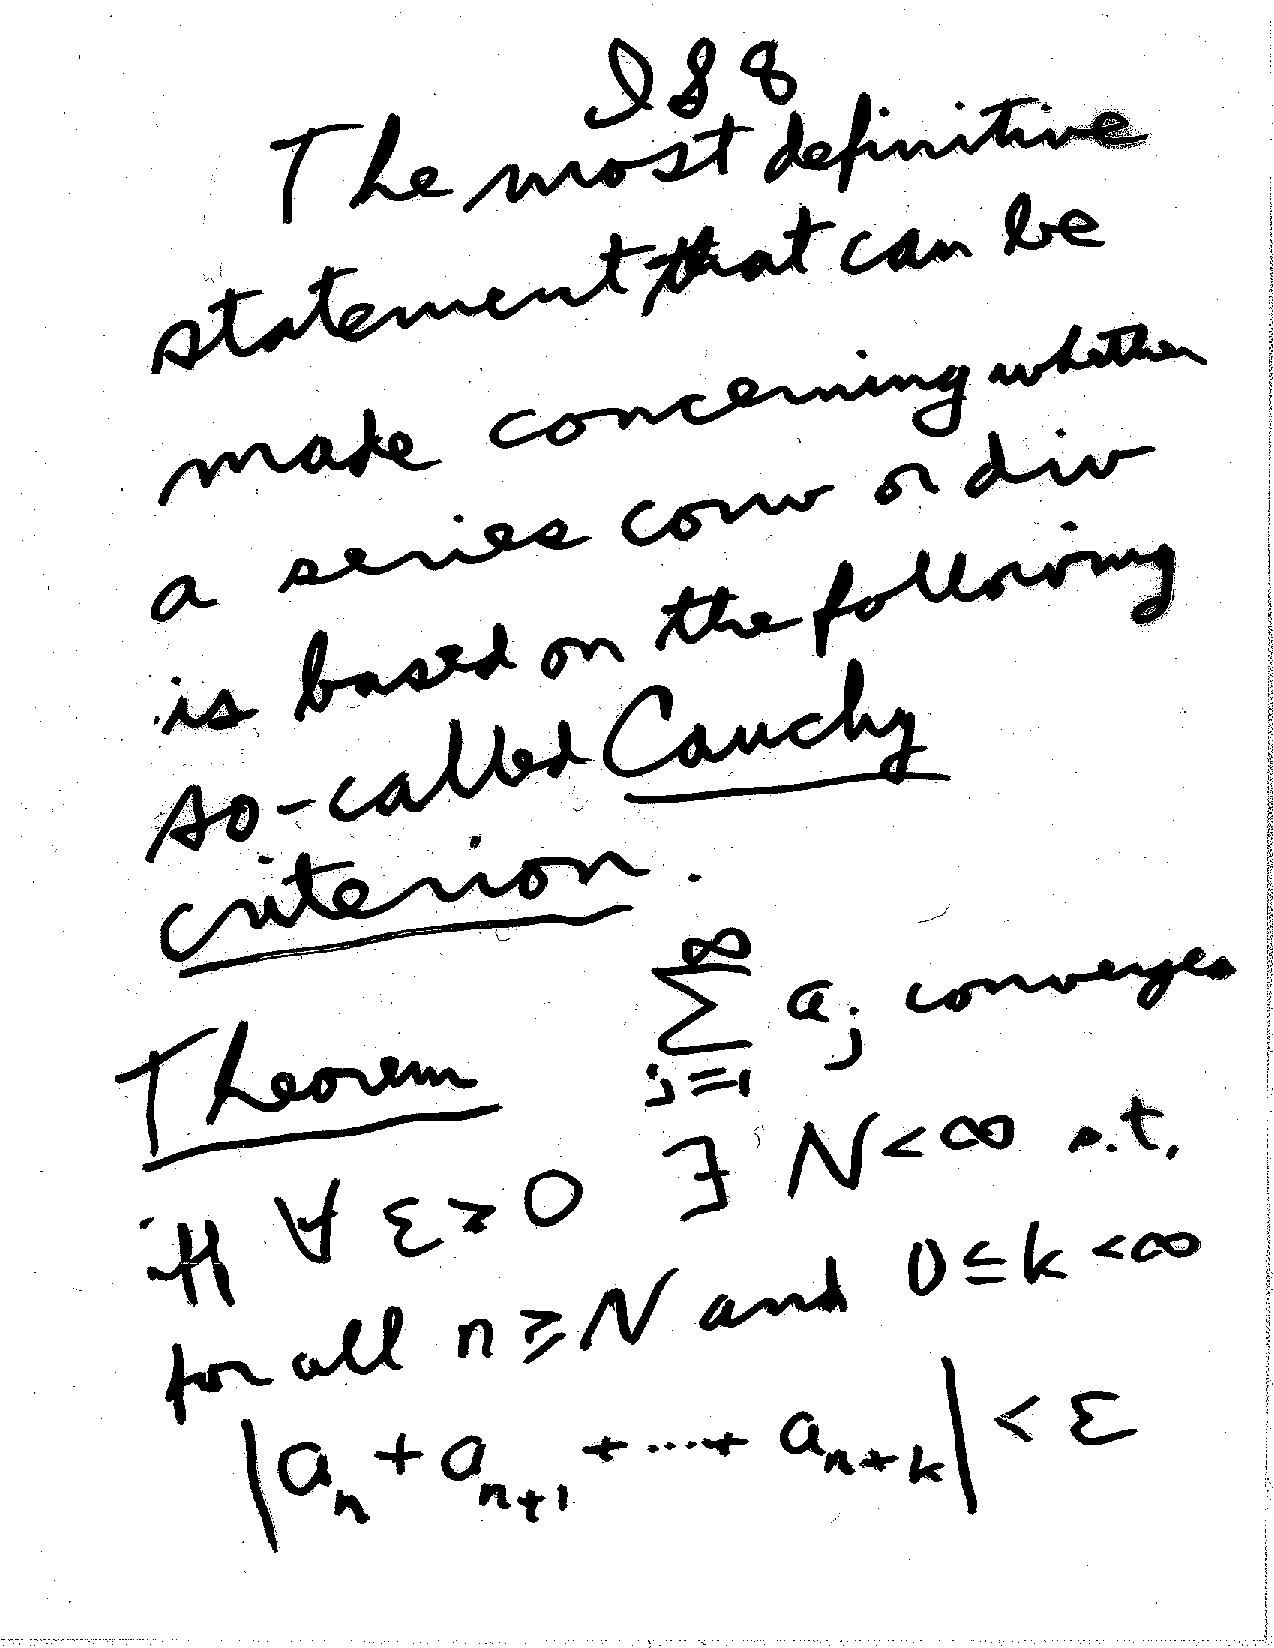
\includegraphics[scale=.5]{Pages/IS_8}

\newpage
 
\begin{center}
IS9
\end{center}

\underline{Pf}: 
Let $S_n = a_1 +...+a_n$
The series converges if $\{s_n\}$ is a Cauchy sequence 

If and only if $\forall \in >$ 0 $\exists$ N $< \infty$ 
Such that for all n $\ge$ N, k $\ge$ 0,
$|s_{n+k} - s_{n-1}|  < \in$ 

Equivalently, if and only if $\forall$ n $\ge$, k $\ge$ 0
$|a_n + a_{n+1} + ... + a_{n+k}| < \in$.

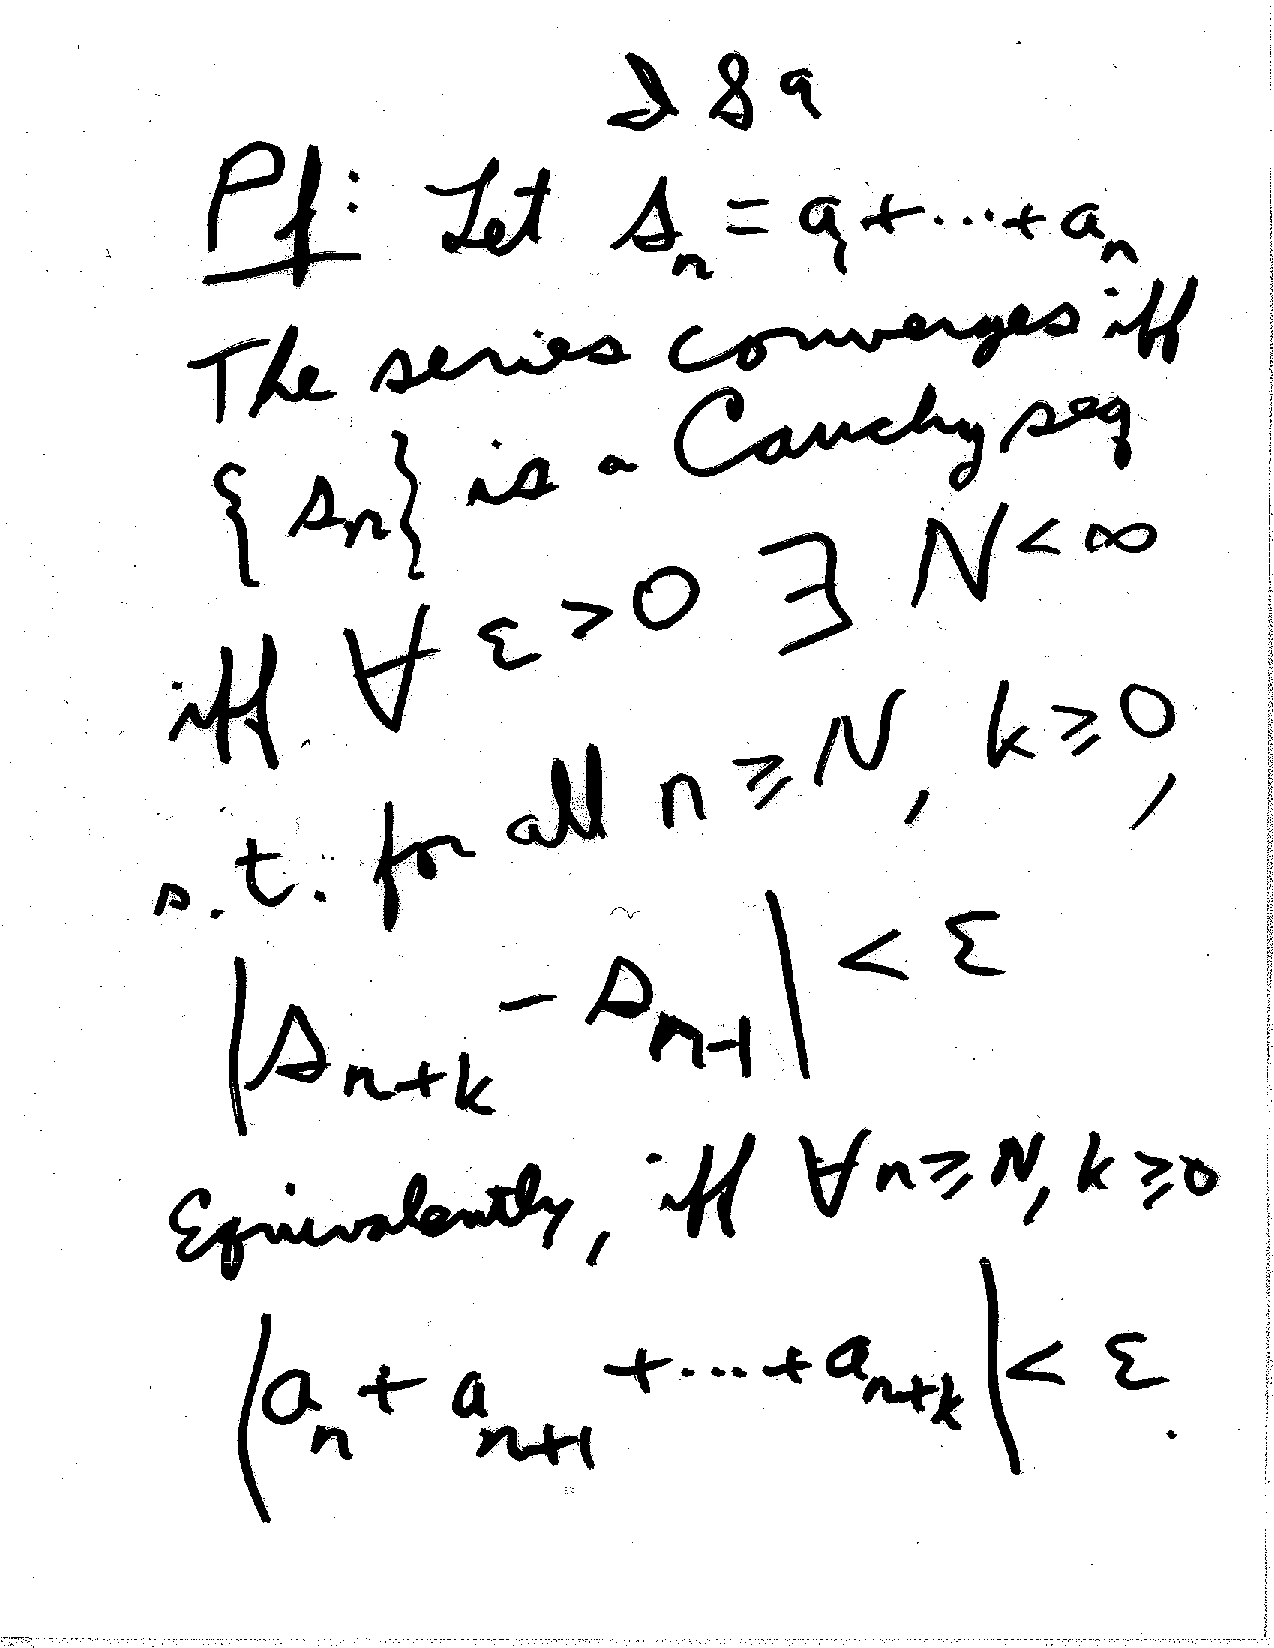
\includegraphics[scale=.5]{Pages/IS_9}

\newpage

\begin{center}
IS10
\end{center}

\underline{Corollary 1} if $\sum_{1}^{\infty} a_j$ converge

then $\lim_{n\to\infty} a_n = 0$

PF: $\lim_{n\to\infty} a_n = \lim_{n\to\infty} (s_n - s_{n-1})$

= 0 if \{$s_n$\} is Cauchy

\underline{Corollary 2} if $\lim_{n\to\infty} |a_n|$

$>$ 0 then $\sum_{1}^{\infty} a_j$ \underline{diverges}

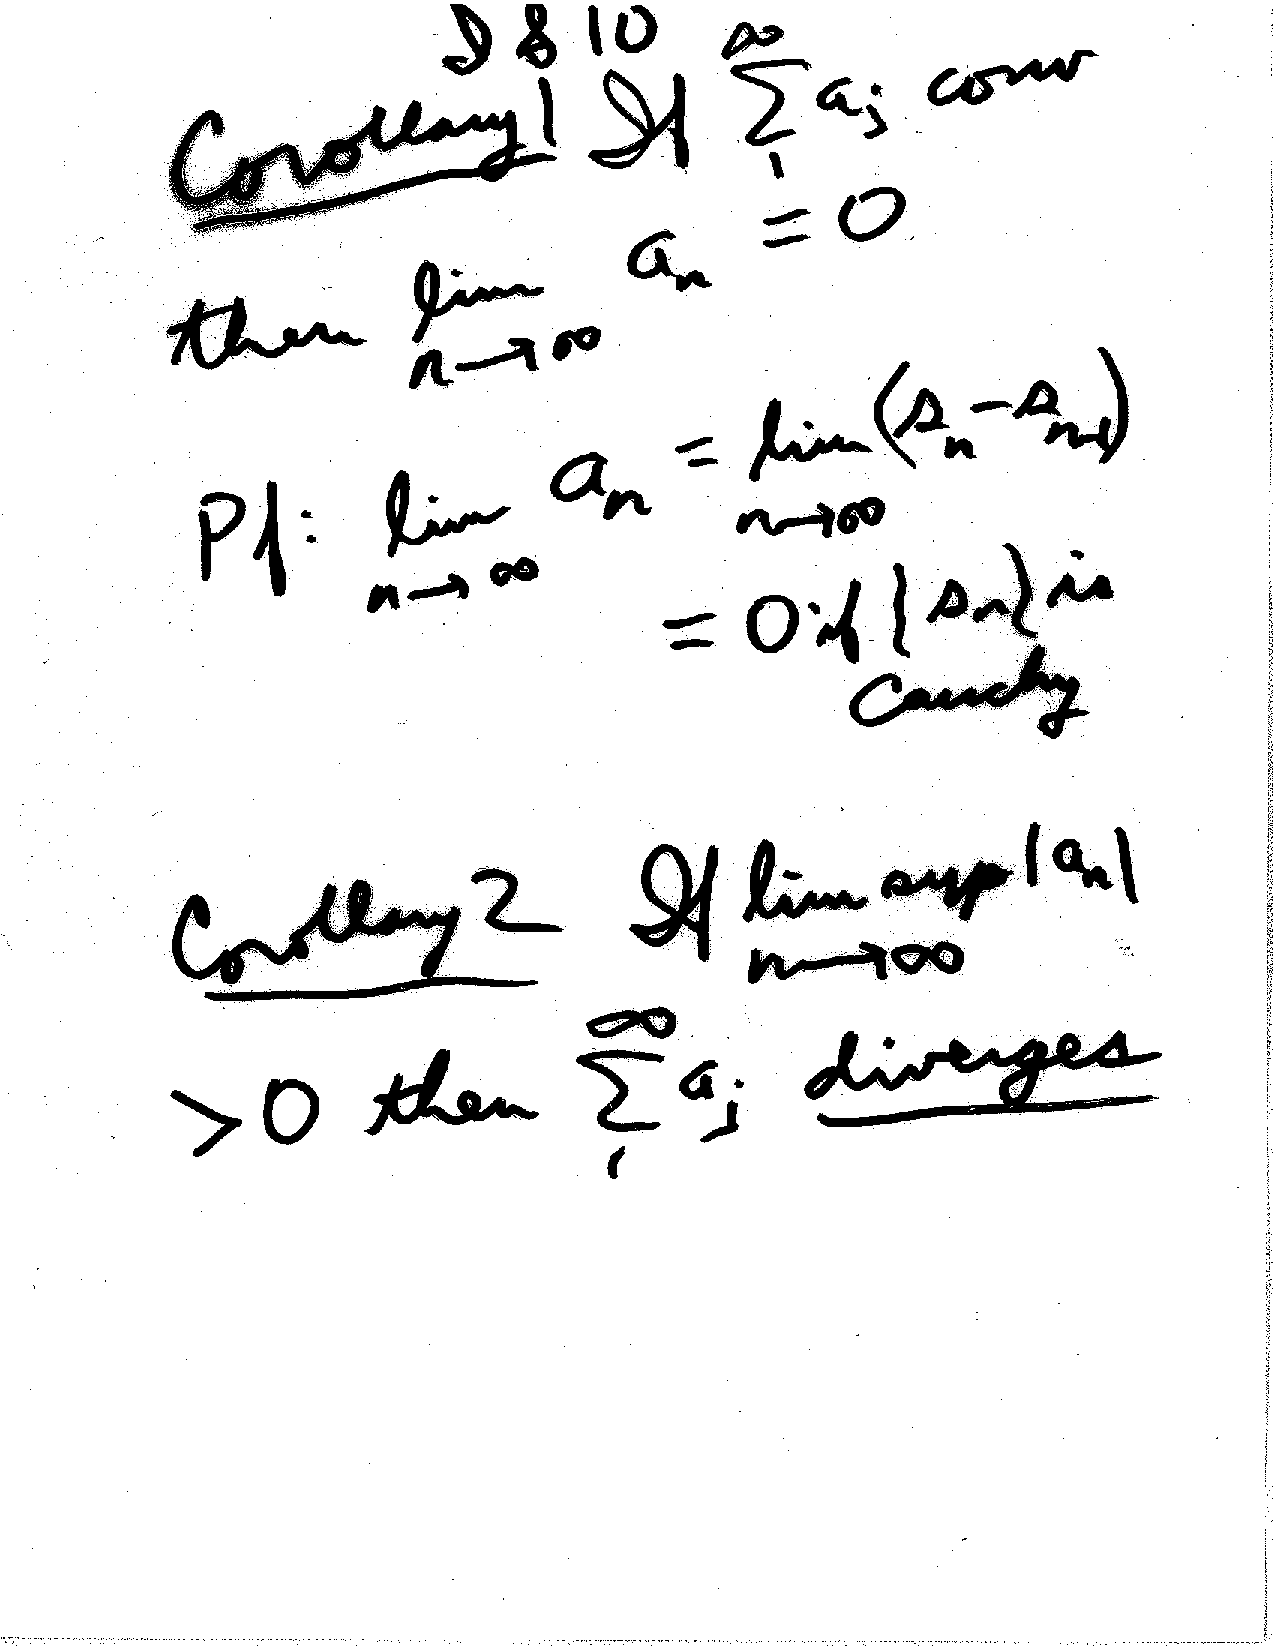
\includegraphics[scale=.5]{Pages/IS_10}

\newpage

\begin{center}
IS11

\underline{Comparison Test}
\end{center}

\underline{Then}
Suppose $|a_n|$ $\le b_n$

Let $S_n$ = $\sum_{j=1}^{n} a_j$ , $T_n = \sum_{j=1}^{n} b_j$

and $\bar{S}_n = \sum_{j=1}^{n}| a_j |$

Then

\begin{enumerate}[i]

\item If  $\lim_{n\to\infty} T_n < \infty$ then $S_n$ and $\bar{S}_n$ converge

\item if $\bar{S}_n$ diverges then $T_n$ diverges
\end{enumerate}

\underline{Def}: 
When $\bar{S}_n < \infty$, $\sum_{}^{\infty}a_j$ is said to converge absolutely

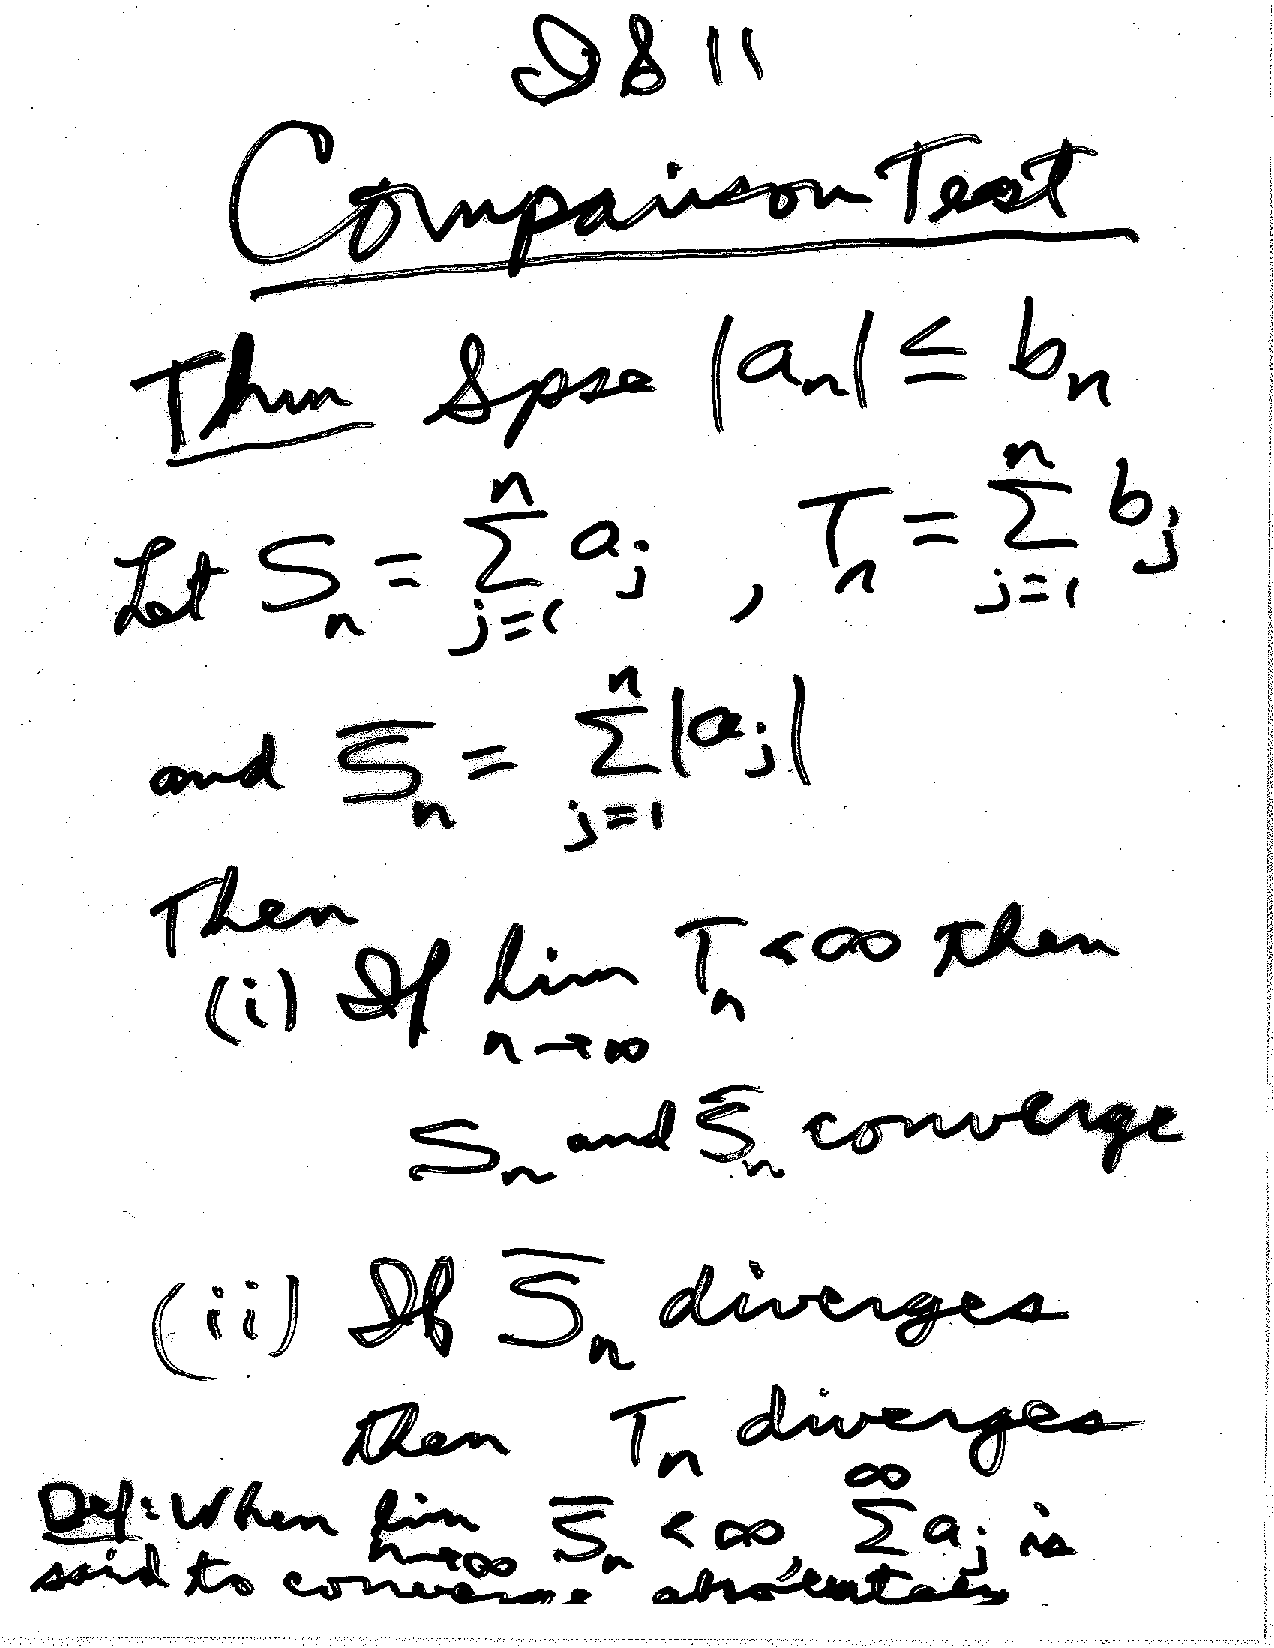
\includegraphics[scale=.5]{Pages/IS_11}

\newpage

\begin{center}
IS12
\end{center}

\underline{Pf}: 
Suppose $T_n$ converges.
 
Fix any $\in > 0$ 

$\exists$ N: $|T_{n+k}-T_n|<\in$ 

    for all n $\ge$ N and k $>$ 0

For such n $\ge$ N and k $>$ 0

$|S_{n+k}-S_n|=|\sum_{n<j \le n+k}^{} a;|$

$\le \sum_{n<j<=n+k}^{} a;|$

$= S_{n+k} - S_n$

$\le \sum_{n<j<=n+k}^{} b;=T_{n+k}-T_n$

$< \in$ hence $S_n$ and $\bar{S}_n$ are Cauchy sequences.

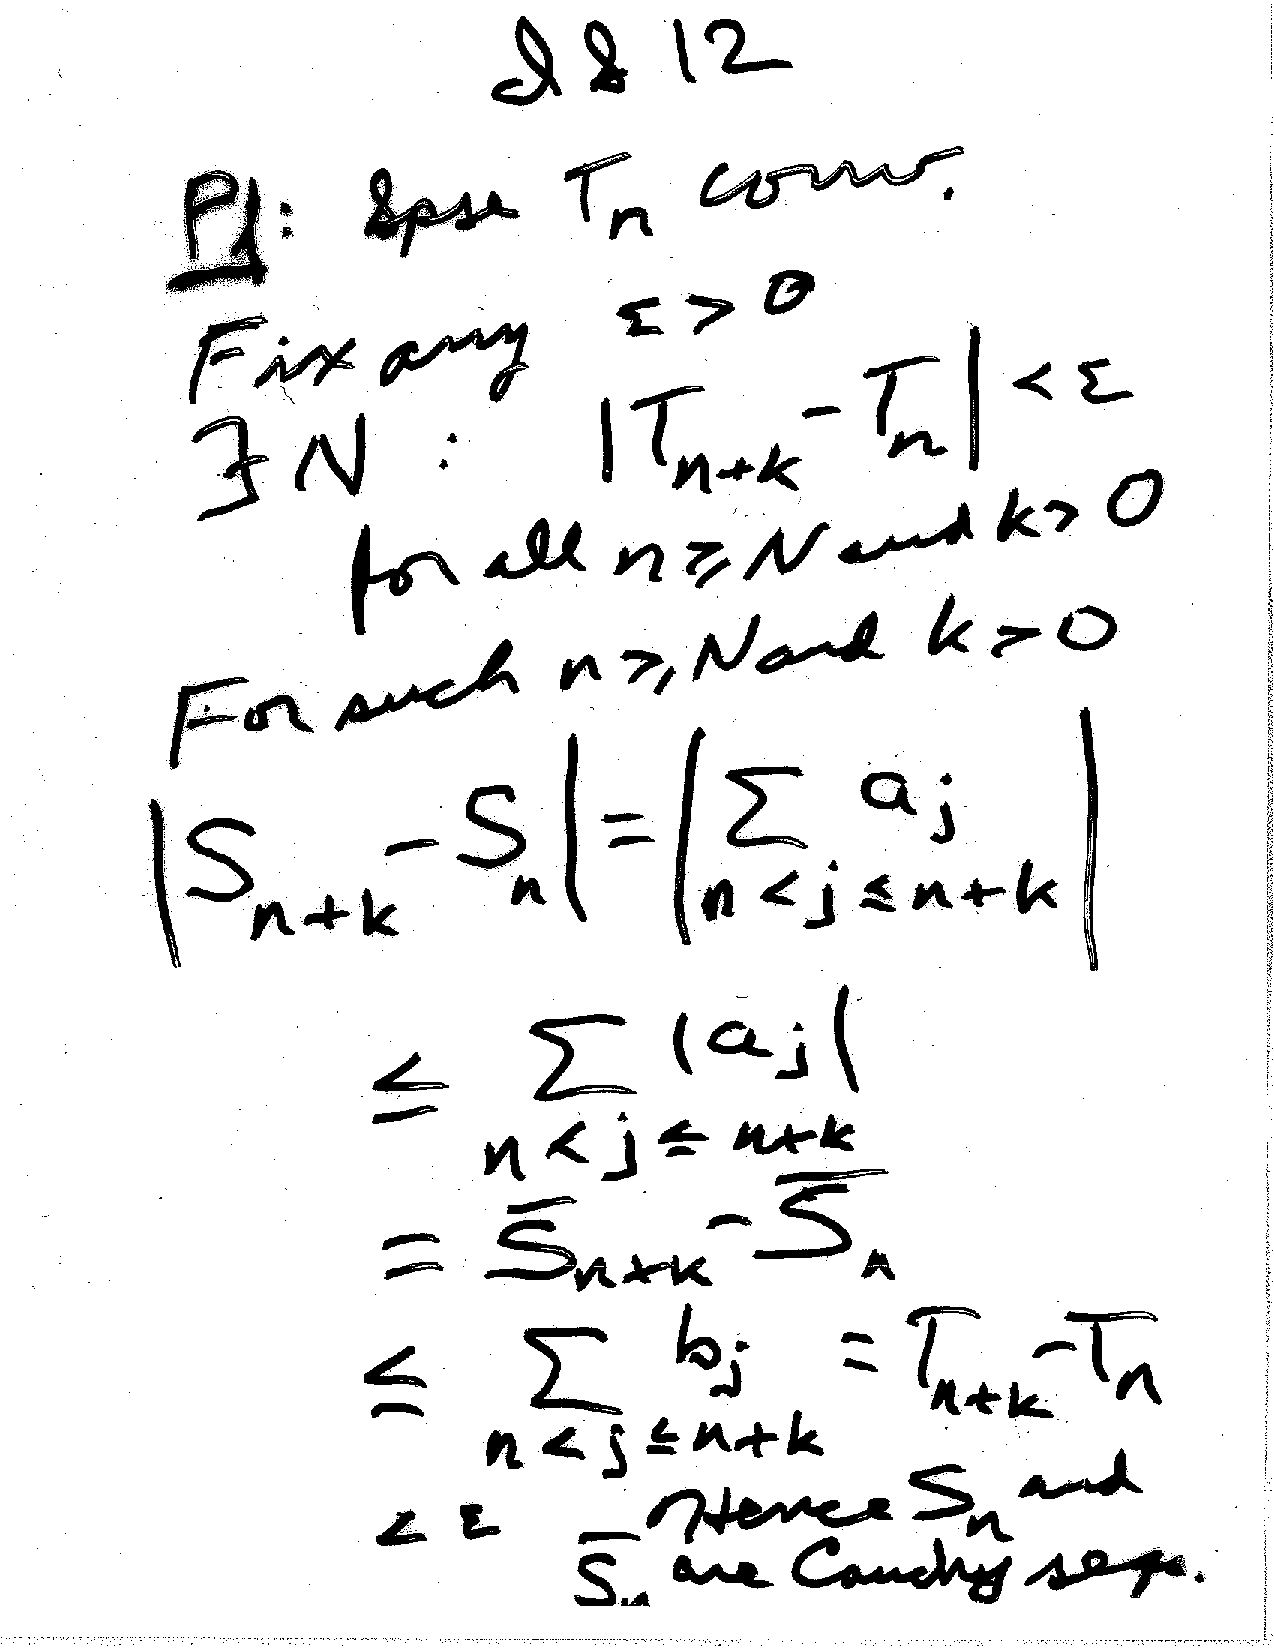
\includegraphics[scale=.5]{Pages/IS_12}

\newpage

\begin{center}
IS13
\end{center}

Therefore $S_n$ and $\bar{S}_n$ converge.

(ii) Suppose $\bar{S}_n$ diverges.

Then $\infty$ = $\lim_{n\to\infty} \bar{S}_n =<\lim_{n\to\infty}T_n$ so \{$T_n$\} diverges.

--------------------------------------------------------------------------------------

For series $s_n$ = $\sum_{j=1}^{n}a_j$
whose terms decrease "like" a geometric series there are a couple of methods of testing for convergence-divergence

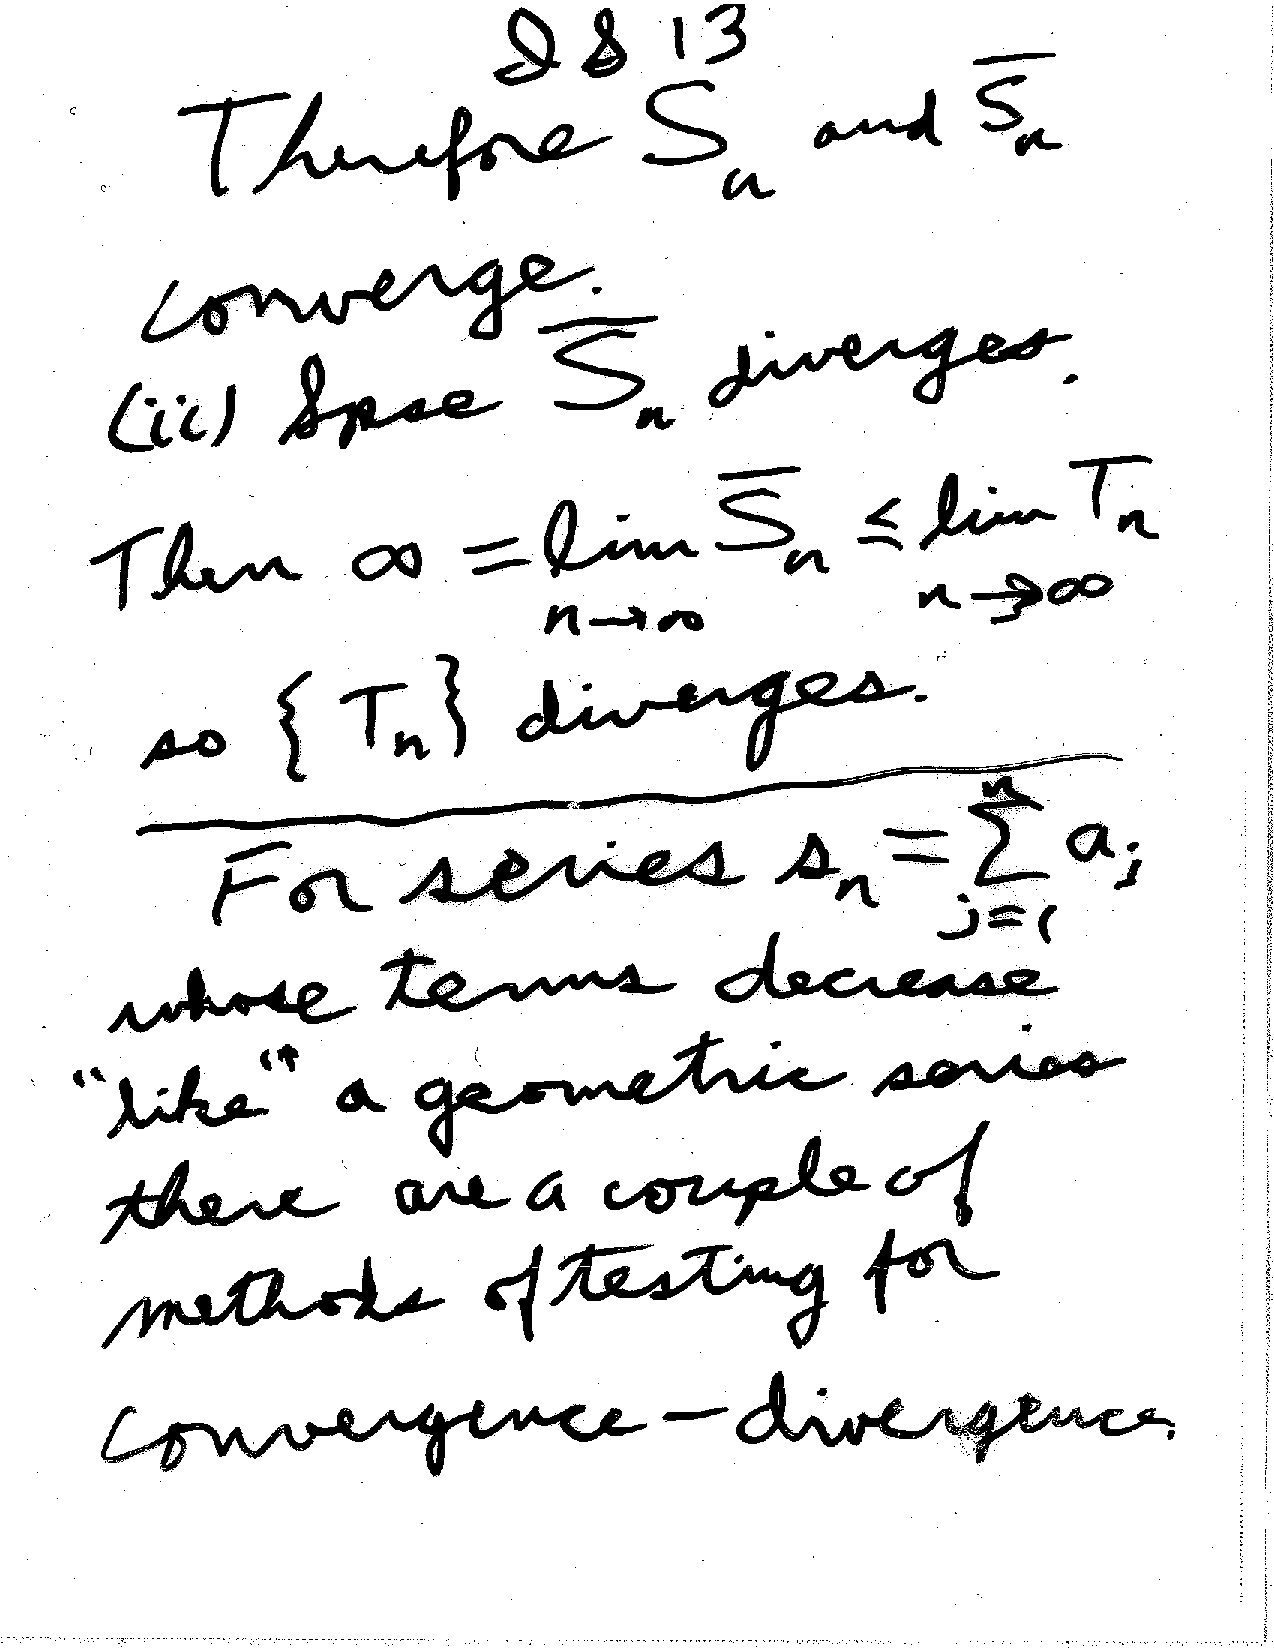
\includegraphics[scale=.5]{Pages/IS_13}

\newpage

\begin{center}
IS14
\end{center}

The simpler is the ratio test

\underline{Then} 
Let $r^* = \bar{\lim_{n\to\infty}} \frac{a_{n+1}}{a_n}$ 

and $r_* =\lim_{n\to\infty} \frac{a_{n+1}}{a_n}$

\begin{enumerate}[i]

\item If $r^*<$1 then $\sum_{n=1}^{\infty}a_n$ \underline{converges absolutely}

\item If $r_* >1$ then $\sum_{n=1}^{n}a_n$ \underline{diverges}

\item If $r_* \le 1 \le r^*$ the test in \underline{not} conclusive

\end{enumerate}

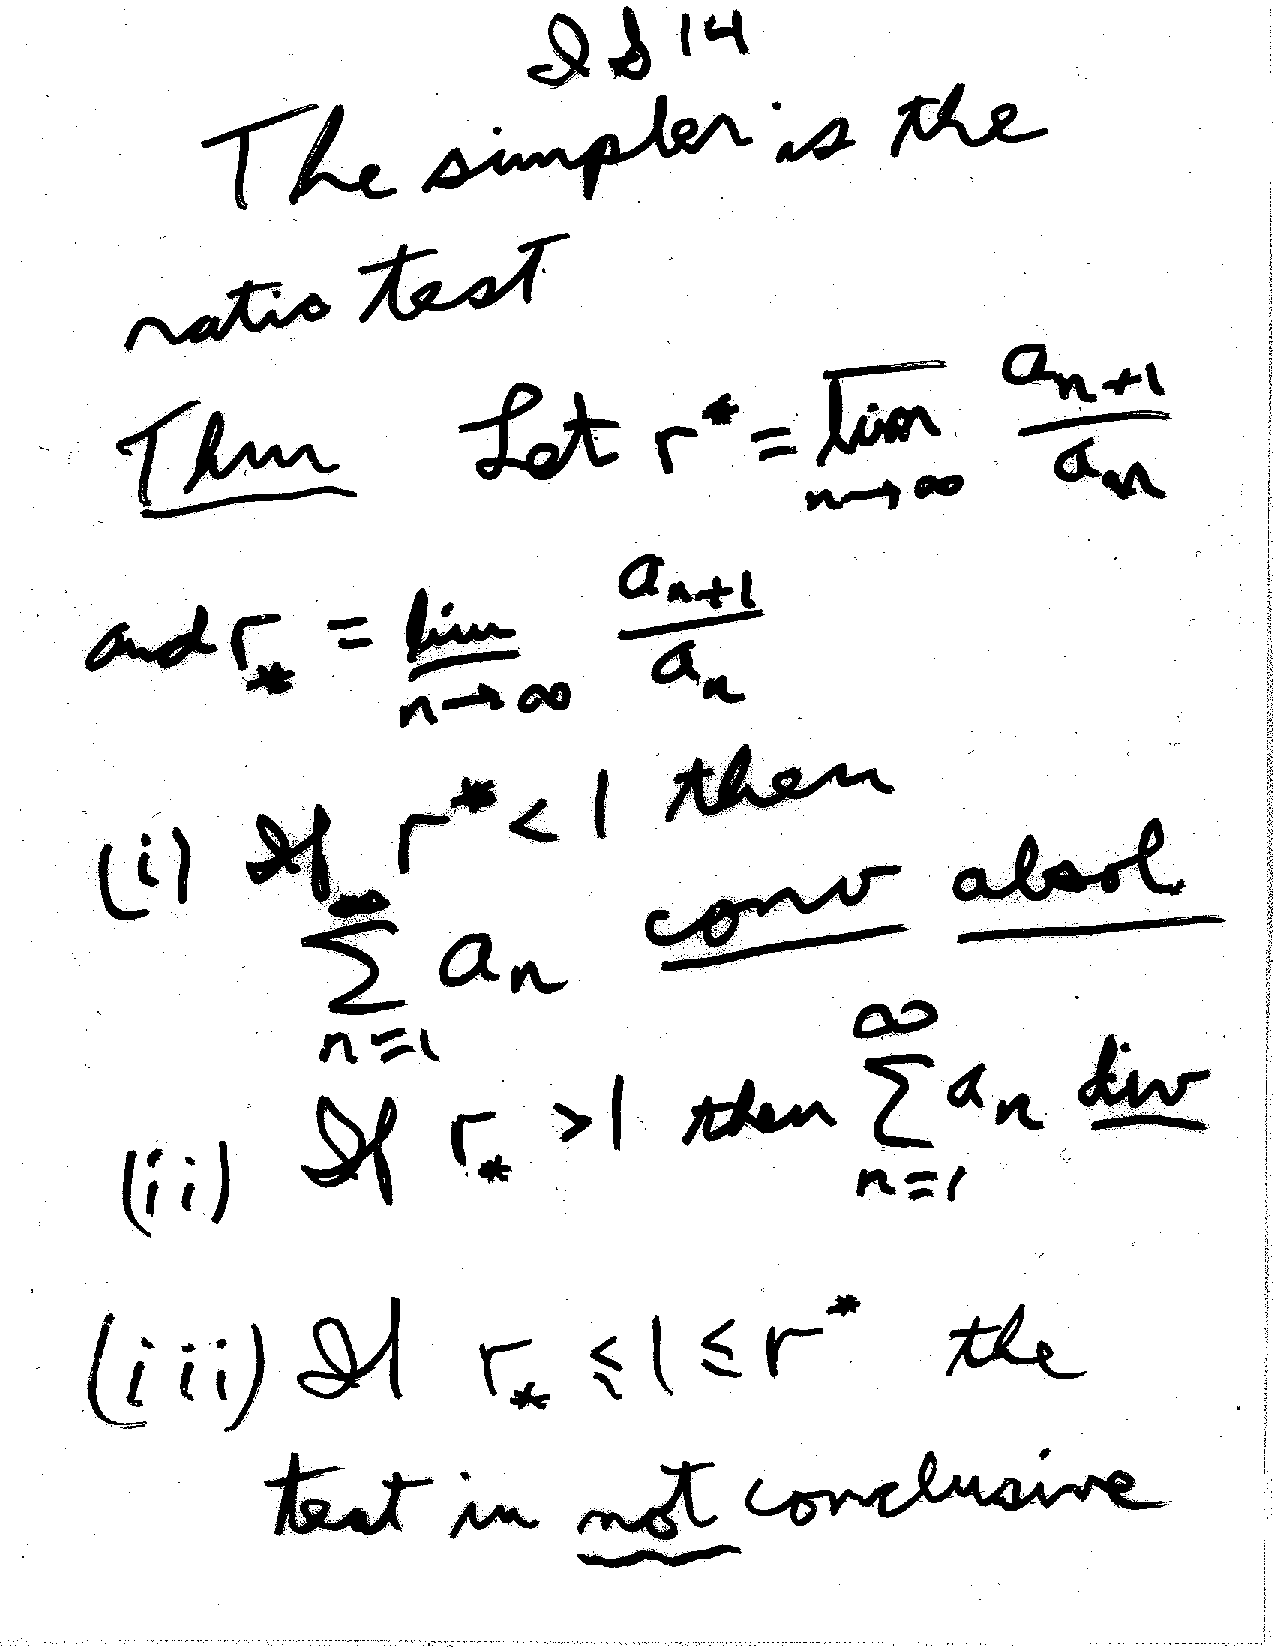
\includegraphics[scale=.5]{Pages/IS_14}

\newpage

\begin{center}
IS15
\end{center}

\underline{Pf}:
Suppose $r^* <1$

Take away $r^* <\lambda <1$

$\exists$ N: for n $>=$ N, $| \frac{a_{n+1}}{a_n} \le \lambda$

$\therefore \sum_{n=N+1}^{\infty}|a_{n}|$

  =$\sum_{k=1}^{\infty}|a_{N+k}|$

  =$\sum_{k=1}^{\infty}|a_{N}|$k $\pi j=1| \frac{a_{N+j}}{a_{N+j-1}}$

  $\le |a_n| \sum_{k=1}^{\infty}|x^k < \infty$ as series converges absolutely.

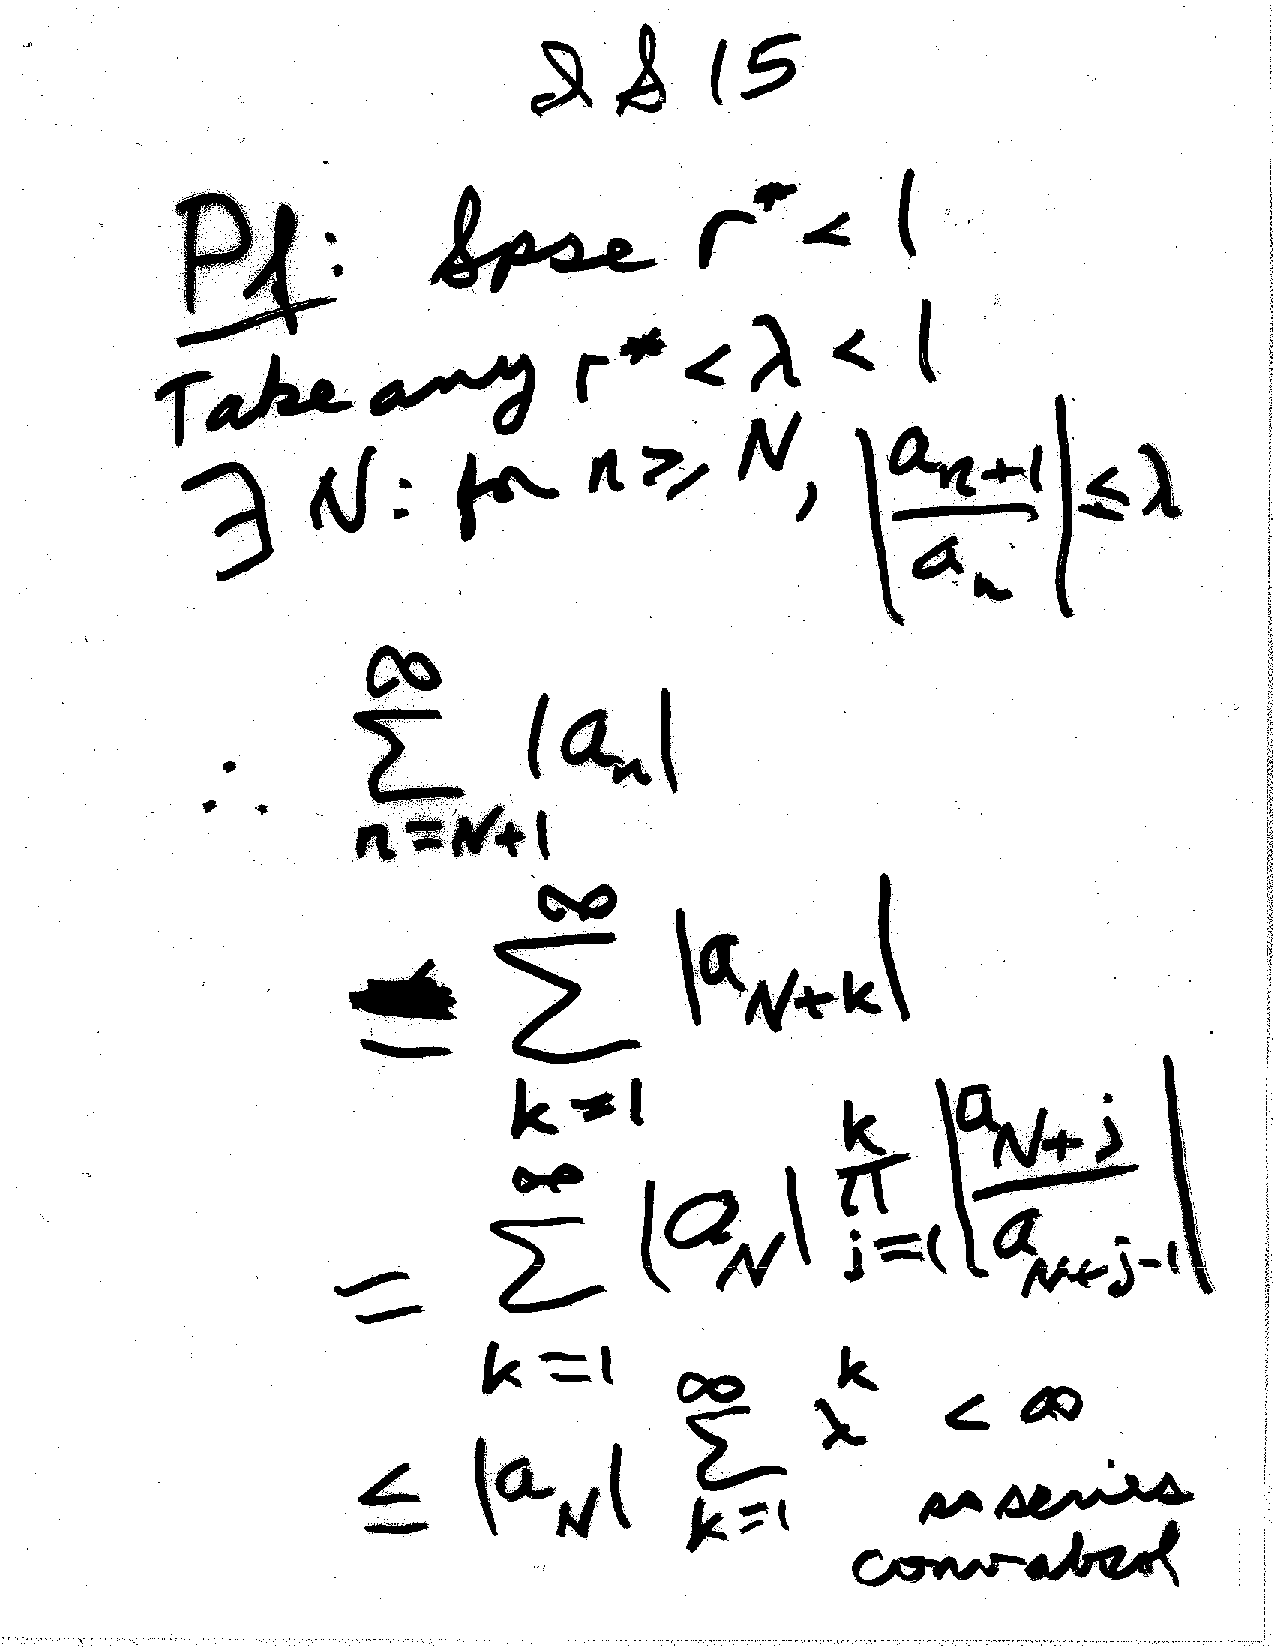
\includegraphics[scale=.5]{Pages/IS_15}

\newpage

%Will: IS16 - IS23

%Rebecca: IS24 - IS32

%Maady: IS33 - IS42

\section{Metric Spaces Part 1}

%Travis: M1 - M5

%Jerome: M6- M10



\section{Metric Spaces Part 2}


%Bryant: M1-M7

%Reshma: M8-M14

%Ethan: M15-M21





\end{document}